% !TEX TS-program = pdflatex
% !TEX encoding = UTF-8 Unicode

% This is a simple template for a LaTeX document using the "article" class.
% See "book", "report", "letter" for other types of document.

\documentclass[11pt]{article} % use larger type; default would be 10pt

\usepackage[utf8]{inputenc} % set input encoding (not needed with XeLaTeX)
\usepackage{hyperref} % Pacote para usar \url

%%% Examples of Article customizations
% These packages are optional, depending whether you want the features they provide.
% See the LaTeX Companion or other references for full information.

%%% PAGE DIMENSIONS
\usepackage{geometry} % to change the page dimensions
\geometry{a4paper} % or letterpaper (US) or a5paper or....
% \geometry{margin=2in} % for example, change the margins to 2 inches all round
% \geometry{landscape} % set up the page for landscape
%   read geometry.pdf for detailed page layout information

\usepackage{graphicx} % support the \includegraphics command and options

% \usepackage[parfill]{parskip} % Activate to begin paragraphs with an empty line rather than an indent

%%% PACKAGES
\usepackage{booktabs} % for much better looking tables
\usepackage{array} % for better arrays (eg matrices) in maths
\usepackage{paralist} % very flexible & customisable lists (eg. enumerate/itemize, etc.)
\usepackage{verbatim} % adds environment for commenting out blocks of text & for better verbatim
\usepackage{subfig} % make it possible to include more than one captioned figure/table in a single float
% These packages are all incorporated in the memoir class to one degree or another...

%%% HEADERS & FOOTERS
\usepackage{fancyhdr} % This should be set AFTER setting up the page geometry
\pagestyle{fancy} % options: empty , plain , fancy
\renewcommand{\headrulewidth}{0pt} % customise the layout...
\lhead{}\chead{}\rhead{}
\lfoot{}\cfoot{\thepage}\rfoot{}

%%% SECTION TITLE APPEARANCE
\usepackage{sectsty}
\allsectionsfont{\sffamily\mdseries\upshape} % (See the fntguide.pdf for font help)
% (This matches ConTeXt defaults)

%%% ToC (table of contents) APPEARANCE
\usepackage[nottoc,notlof,notlot]{tocbibind} % Put the bibliography in the ToC
\usepackage[titles,subfigure]{tocloft} % Alter the style of the Table of Contents
\renewcommand{\cftsecfont}{\rmfamily\mdseries\upshape}
\renewcommand{\cftsecpagefont}{\rmfamily\mdseries\upshape} % No bold!

%%% END Article customizations


\title{ANÁLISE DA EFICIÊNCIA E PRATICIDADE NA IMPLEMENTAÇÃO DE OPERAÇÕES CRUD UTILIZANDO A LINGUAGEM PYTHON COM DJANGO: UM ESTUDO SOBRE DESEMPENHO E FLEXIBILIDADE EM FRAMEWORKS WEB}
\author{Antônio Fernandes De Santana Neto\\ Manoel Dantas Macedo Filho \\ Universidade Tiradentes - UNIT}
\date{25/11/2024} 

\begin{document}


\maketitle
\begin{abstract}
Este artigo explora a eficiência e praticidade na implementação de operações CRUD (Create, Read, Update, Delete) utilizando a linguagem Python e o framework Django no desenvolvimento de aplicações web. Através de uma análise detalhada, são discutidos os aspectos técnicos que tornam o Django uma escolha robusta para a criação e gestão de sistemas de persistência de dados. Além de fornecer um guia prático, o artigo examina a flexibilidade e o desempenho do Django na execução de operações CRUD, destacando como sua arquitetura permite a rápida implementação e escalabilidade de aplicações web. Este estudo busca capacitar desenvolvedores a compreender as vantagens técnicas e as considerações práticas na escolha de tecnologias para projetos que demandam alta eficiência e manutenibilidade.\\
Palavras chave: CRUD, Python, Django, Desenvolvimento Web, Persistência de Dados, Eficiência, Flexibilidade. \\

This article explores the efficiency and practicality of implementing CRUD (Create, Read, Update, Delete) operations using the Python language and the Django framework in the development of web applications. Through a detailed analysis, the technical aspects that make Django a robust choice for creating and managing data persistence systems are explained. In addition to providing a practical guide, the article examines the flexibility and performance of Django in executing CRUD operations, highlighting how its architecture allows for the rapid implementation and scalability of web applications. This study aims to enable developers to understand the technical advantages and practical considerations in choosing technologies for projects that require high efficiency and maintainability.\\ 
Keywords: CRUD, Python, Django, Web Development, Data Persistence, Efficiency, Flexibility.\\
\end{abstract}


\maketitle
\section{Introdução}
No desenvolvimento de aplicações web, a manipulação eficiente de dados é fundamental para garantir a integridade e a funcionalidade dos serviços oferecidos. As operações CRUD (Create, Read, Update, Delete) representam a base do gerenciamento de dados, permitindo que informações sejam criadas, lidas, atualizadas e excluídas de maneira organizada e eficaz. Segundo a Mozilla Developer Network, “CRUD é um acrônimo para as maneiras de operar dados armazenados, e representa as quatro funções básicas do armazenamento persistente.”
 \\\\
O Django, um dos frameworks mais populares para Python, se destaca por oferecer um conjunto robusto de ferramentas que facilitam a implementação dessas operações em qualquer aplicação web. Este artigo tem como objetivo geral analisar como o Django, aliado ao Python, permite a construção eficiente e flexível de um sistema CRUD, com foco na rapidez de desenvolvimento e na adaptabilidade às necessidades específicas de diferentes projetos.
\\\\
Já os Objetivos Específicos transitam entre os seguintes interesses: “Demonstrar a implementação prática de um CRUD utilizando Django, explorando as etapas de criação, leitura, atualização e exclusão de dados”; “Avaliar como o Django facilita a integração de regras de negócio complexas, mantendo a estrutura do código clara e organizada”; “Analisar a eficiência do Django em termos de desempenho e facilidade de manutenção, especialmente no contexto de aplicações escaláveis”; e “Investigar a flexibilidade do Django na adaptação de sistemas CRUD para diferentes cenários de aplicação, desde pequenas soluções até sistemas de grande porte. 
\\\\
A Justificativa na escolha de Python e Django para este estudo se dá pela ampla adoção dessas tecnologias na indústria de desenvolvimento web, motivada por sua combinação de simplicidade e poder. Python é reconhecido por sua clareza e facilidade de aprendizado, enquanto o Django se destaca por sua abordagem completa, que inclui um vasto conjunto de funcionalidades prontas para uso. A análise apresentada neste artigo visa preencher uma lacuna na literatura técnica, ao oferecer tanto um guia prático quanto uma análise aprofundada das capacidades do Django, especialmente em comparação com outros frameworks. Dessa forma, o artigo busca capacitar desenvolvedores a escolherem as ferramentas mais adequadas para implementar sistemas CRUD que sejam ao mesmo tempo eficientes, escaláveis e fáceis de manter.

\maketitle \section{Fundamentação Teórica}
A eficiência e a praticidade na implementação de operações CRUD são aspectos cruciais no desenvolvimento de sistemas web modernos, especialmente em contextos onde a escalabilidade e a manutenibilidade são requisitos indispensáveis. Esses dois conceitos, embora distintos, estão profundamente interligados quando se trata da escolha de tecnologias e frameworks para o desenvolvimento web.

\subsection{Eficiência no Desenvolvimento Web}
A eficiência no desenvolvimento web refere-se à capacidade de um sistema em executar operações de maneira rápida e com baixo consumo de recursos. No contexto das operações CRUD, essa eficiência é medida pela rapidez com que o sistema pode processar solicitações de criação, leitura, atualização e exclusão de dados. Além disso, a eficiência também envolve o uso otimizado de recursos como memória, CPU e I/O (entrada e saída), que são críticos em sistemas que necessitam de alta disponibilidade e baixo tempo de resposta. 
\\\\
O Django, como um framework de alto nível para Python, oferece uma série de ferramentas e otimizações que contribuem para essa eficiência. A utilização de ORM (Object-Relational Mapping), por exemplo, permite que desenvolvedores manipulem bancos de dados de forma mais intuitiva e eficiente, sem a necessidade de escrever consultas SQL complexas. Estudos como o de Silva et al. (2020) destacam que a abstração proporcionada pelo ORM do Django pode reduzir significativamente o tempo de desenvolvimento e minimizar erros relacionados à manipulação direta do banco de dados.

\subsection{Praticidade e Flexibilidade no Uso de Frameworks}
Praticidade no desenvolvimento refere-se à facilidade e rapidez com que os desenvolvedores podem implementar funcionalidades, adaptar o sistema a novos requisitos e manter o código ao longo do tempo. Um framework é considerado prático quando ele reduz a complexidade do código, promove a reutilização e facilita a integração de novas funcionalidades sem comprometer a estrutura existente do sistema. 
\\\\
O Django se destaca por sua abordagem "batteries-included", que significa que ele vem com uma série de funcionalidades pré-configuradas e prontas para uso. Isso inclui um sistema de autenticação robusto, um painel administrativo automático e ferramentas para a criação de APIs RESTful. Essa característica permite que desenvolvedores concentrem seus esforços na lógica de negócios específica da aplicação, ao invés de reinventar soluções comuns. 
\\\\
Além disso, a flexibilidade do Django é outro ponto chave. O framework permite que as operações CRUD sejam personalizadas para atender a requisitos específicos, seja pela modificação de comportamentos padrão ou pela integração de pacotes externos. O uso de mixins e viewsets no Django REST Framework, por exemplo, facilita a criação de APIs customizadas, que podem ser ajustadas para oferecer o equilíbrio ideal entre desempenho e funcionalidade.

\subsection{Versatilidade e Aplicabilidade em Diferentes Cenários}
Uma das grandes vantagens do Django é a sua versatilidade, que permite que aplicações desenvolvidas com esse framework sejam adaptadas para uma ampla variedade de cenários e regras de negócio. Essa versatilidade é possível graças à arquitetura modular do Django, que permite que os desenvolvedores adicionem ou removam funcionalidades conforme necessário, ajustando a aplicação às demandas específicas de diferentes projetos. 
\\\\
Por exemplo, uma aplicação CRUD desenvolvida em Django pode ser facilmente adaptada para atender a diferentes setores, como e-commerce, educação, saúde, entre outros. A principal estrutura de dados e operações permanece consistente, enquanto as regras de negócio específicas podem ser customizadas através da implementação de modelos personalizados, formulários, e lógica de backend. Esse nível de customização é facilitado pelo uso de Django signals, middleware, e a robusta API de modelagem. 
\\\\
Além disso, o painel administrativo nativo do Django é uma ferramenta poderosa que torna a aplicação facilmente auditável e gerenciável. Esse painel permite que os administradores monitorem e gerenciem o sistema de maneira intuitiva, o que é especialmente útil em ambientes onde a integridade e a segurança dos dados são críticas. A capacidade de auditar e ajustar rapidamente as operações através do painel administrativo torna o Django uma escolha atrativa para projetos que exigem flexibilidade e adaptabilidade.
\\\\
Essa capacidade de adaptação é crucial para garantir que a aplicação possa evoluir com as necessidades do negócio, permitindo que o mesmo código base seja reutilizado em diferentes contextos com ajustes mínimos. A robustez do Django, combinada com sua flexibilidade, possibilita a criação de soluções que são ao mesmo tempo específicas para um contexto e escaláveis para atender novas demandas.

\subsection{Comparação com Outros Frameworks}
Embora o Django seja amplamente reconhecido por sua eficiência e praticidade, é importante considerar como ele se compara a outros frameworks. Frameworks como Flask (para Python) e Laravel (para PHP) são frequentemente mencionados em comparações devido à sua simplicidade e flexibilidade. No entanto, a escolha entre Django e outros frameworks deve ser guiada pelos requisitos específicos do projeto. O Django é geralmente preferido em projetos que demandam uma estrutura mais rígida e que precisam escalar rapidamente, enquanto o Flask pode ser mais adequado para aplicações menores e mais flexíveis.
 \\\\
A análise teórica apresentada aqui estabelece a base para a discussão prática que será abordada na metodologia deste estudo. Ao entender os princípios de eficiência, praticidade, e versatilidade no uso de frameworks como Django, desenvolvedores podem fazer escolhas mais informadas que impactam diretamente a qualidade e o sucesso de seus projetos.


\maketitle
\section{Metodologia}
Este artigo tem como foco a implementação de um sistema de gerenciamento de usuários que abrange todas as operações CRUD (Create, Read, Update, Delete) de maneira visual e de fácil compreensão. Para facilitar a interação com o sistema, será criado um "superusuário" que possui permissões administrativas completas, permitindo a gestão de outros usuários dentro da aplicação. Essa abordagem é fundamental para garantir que os administradores possam realizar operações essenciais, como a criação de novos usuários, a leitura de informações, a atualização de dados existentes e a exclusão de usuários que não sejam mais necessários. 
\\\\
O desenvolvimento do sistema seguirá uma metodologia estruturada, começando pela configuração do ambiente de desenvolvimento com Python e Django. Inicialmente, será necessário instalar as dependências necessárias e configurar o banco de dados, que servirá como a base para a persistência de dados. Em seguida, serão definidas as rotas e as views que permitirão a interação do usuário com o sistema, garantindo que todas as operações CRUD sejam implementadas de maneira eficiente e intuitiva.
 \\\\
Além disso, o sistema contará com a implementação de formulários que facilitarão a entrada de dados e a validação das informações fornecidas pelos usuários. Os formulários serão projetados para serem amigáveis, garantindo que os administradores tenham uma experiência fluida ao inserir ou modificar dados. Assim, será possível validar as informações em tempo real e fornecer feedback imediato, o que é crucial para a manutenção da integridade dos dados. 
\\\\
Embora este artigo não aborde a criação de "grupos de usuários", é importante destacar que essa funcionalidade é facilmente integrável ao sistema. A adição de grupos de usuários permitirá uma auditoria e um controle de permissões mais granulares, possibilitando a segmentação de acessos e a definição de diferentes níveis de permissão para cada grupo. Essa flexibilidade é um dos grandes benefícios do uso do Django, pois permite que o sistema se adapte às necessidades específicas de cada aplicação, garantindo a escalabilidade e a robustez necessárias para um gerenciamento eficaz de dados.


\maketitle
\section{Desenvolvimento}
O processo de desenvolvimento deste sistema CRUD pode se basear em três pilares bem relevantes nesse contexto: a configuração do ambiente de desenvolvimento, a criação das rotas e views, e a implementação dos formulários para manipulação de dados. Estes passos garantem que todas as operações (Create, Read, Update, Delete) sejam realizadas de forma eficiente e com uma interface intuitiva. \\\\
Sobre a configuração do Ambiente de Desenvolvimento, o primeiro passo para iniciar o projeto deve ser, claro, configurar o ambiente de desenvolvimento e, se for utilizar o Django é necessário instalar as dependências básicas, incluindo o Python e o Django por meio do gerenciador de pacotes pip. Além disso, foi configurado o banco de dados SQLite, uma escolha apropriada para o projeto, devido à sua simplicidade e eficiência em aplicações de pequeno porte. A conexão ao banco de dados foi mantida com o padrão no arquivo settings.py, garantindo que a aplicação pudesse persistir dados, o que a um projeto pequeno é mais que suficiente. \\\\
Assim, o foco do artigo é criar uma aplicação simples, mantendo as features básicas já contidas no Django, mostrando como utilizar e gerenciar as funcionalidades com seu determinado fim.
\subsection{Sistema Operacional}
A escolha do Linux como sistema operacional base para o desenvolvimento deste projeto reflete a sua popularidade e confiabilidade entre desenvolvedores de software. O Linux, especialmente na distribuição Debian, oferece um ambiente estável e seguro, com suporte robusto para Python e Django. Além disso, seu modelo de código aberto permite uma flexibilidade significativa, crucial para um desenvolvimento ágil e voltado para a personalização. Este ambiente favorece o controle total sobre o sistema, algo essencial para aplicações web que exigem um gerenciamento eficiente de recursos e segurança. Neste artigo, foi utilizado o sistema operacional Linux, especificamente a versão Debian 5.10.0-18-amd64 (SMP Debian 5.10.140-1, lançado em 02 de setembro de 2022, arquitetura x86-64).
\subsection{Python 3.11.9}
A versão 3.11.9 do Python foi escolhida devido a melhorias em performance e suporte a recursos modernos da linguagem, que otimizam a implementação de sistemas complexos. O Python é amplamente adotado pela comunidade de desenvolvedores por sua sintaxe limpa e clara, facilitando a escrita e manutenção de código. Além disso, as bibliotecas disponíveis e o vasto ecossistema tornam o Python uma excelente escolha para desenvolvimento web com o Django, por exemplo.

\maketitle
\section{Implementação}
\subsection{Criaçao do diretório}
A organização do projeto começa com a criação de uma estrutura de diretórios clara, que facilita o gerenciamento de arquivos e a separação lógica dos componentes do sistema. Para fins de organização, foi criado uma pasta chamada "crud" e posteriormente adentrado na mesma, como ilustra a imagem a seguir:\\\\
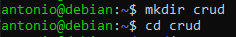
\includegraphics[]{images/s1.PNG}
\subsection{Ambiente Virtual}
O uso de um ambiente virtual (venv) é uma prática essencial no desenvolvimento de aplicações Python, garantindo que as dependências de cada projeto sejam isoladas, evitando conflitos entre pacotes instalados globalmente e os requisitos específicos do projeto. Além de proporcionar organização, o ambiente virtual melhora a reprodutibilidade do ambiente de desenvolvimento, permitindo que outros desenvolvedores ou sistemas possam replicar a configuração de forma precisa. Dito isto, foi criado um ambiente virtual onde instalaremos o Django e todas suas respectivas dependências.\\\\
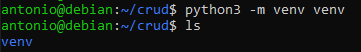
\includegraphics[]{images/s2.PNG}\\\\
Depois de criar o ambiente virtual, iremos ativar o mesmo:\\\\
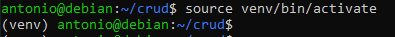
\includegraphics[]{images/s3.PNG}
\subsection{Django}
\subsubsection{Instalação}
A instalação do Django em um ambiente virtual, utilizando o gerenciador de pacotes pip, demonstra a simplicidade com que se pode iniciar o desenvolvimento de aplicações web com este framework. A grande vantagem do Django é sua abordagem "batteries included", ou seja, ele vem com uma série de funcionalidades prontas, como autenticação, administração e ORM, permitindo ao desenvolvedor focar na lógica de negócios sem se preocupar com detalhes de infraestrutura e configurações mais genéricas. \\\\
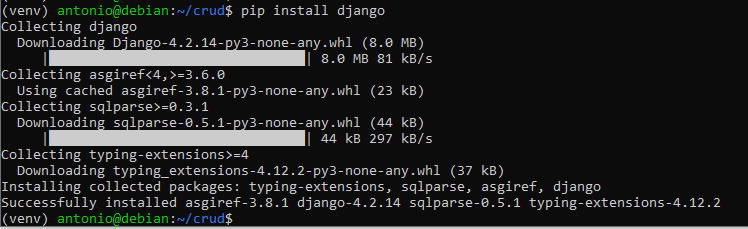
\includegraphics[width=150mm,scale=1]{images/s4.PNG}
\subsubsection{Criação da aplicação}
A criação do projeto com o comando django-admin startproject dá início à estrutura base da aplicação. O Django organiza automaticamente os arquivos principais e as configurações, facilitando o início do desenvolvimento. Esse processo automatizado economiza tempo e esforço, permitindo que o desenvolvedor comece a trabalhar na lógica da aplicação imediatamente, pois arquitetura base e integrações com o banco de dados já vêm previamente prontas.\\\\
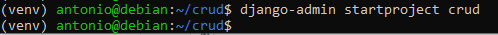
\includegraphics[]{images/s5.PNG}
\subsubsection{Migrations}
Migrations no Django são uma funcionalidade essencial para o gerenciamento e evolução de bancos de dados durante o ciclo de vida de uma aplicação. Elas permitem que qualquer alteração feita nos modelos de dados — como a criação de novas tabelas, a adição de colunas, ou a modificação de tipos de dados — seja registrada e aplicada de forma automática e ordenada no banco de dados.\\\\
Cada vez que o desenvolvedor faz uma alteração nos models (que representam a estrutura de dados da aplicação), o Django gera arquivos de migrations, que documentam essas mudanças. Essas migrations garantem que o banco de dados esteja sempre atualizado com a versão mais recente do código, mantendo uma correspondência precisa entre a camada de aplicação e a camada de persistência de dados.\\\\
Com a aplicação já criada, precisamos modelar o banco de dados que armazenará as informações utilizando os migrations. "Migrations são a maneira do Django de propagar as alterações feitas em seus Models (adicionando um campo, excluindo um modelo, etc.) em seu esquema de banco de dados." (Documentação oficial do Django). Estes "Models" são arquivos criados manualmente pelo desenvolvedor para modular alguma tabela do banco de dados, todavia existem algumas que já vem por padrão criadas, dentre elas, o Model de "User" (usuário). Então podemos aplicar os arquivos de migrations que já vem com o framework e teremos o banco de dados modularizados para auditar usuários.\\\\
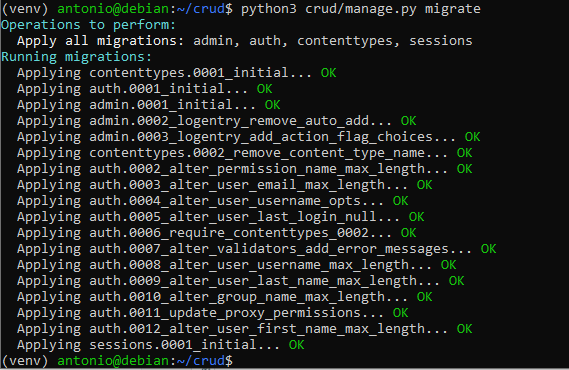
\includegraphics[]{images/s6.PNG}
\subsubsection{Super Usuário}
A criação de um superusuário no Django é uma etapa fundamental, pois garante o acesso administrativo ao sistema. Com o superusuário, é possível gerenciar todas as funcionalidades da aplicação, como a criação, atualização e remoção de usuários e dados. Essa funcionalidade de auditoria e controle é crucial para sistemas em produção, pois oferece uma camada adicional de facilidade para o gerenciamento.
Quando todas as aplicações dos arquivos de Migrations forem aplicados, poderemos criar o "super usuário" que auditará toda e qualquer informação do sistema. Neste caso foi criado com o nome de usuário "root" e senha "root".\\\\
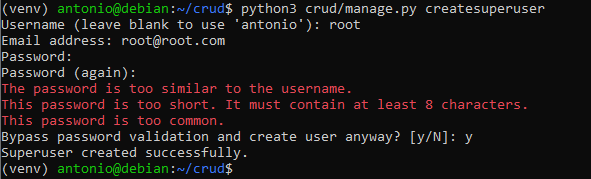
\includegraphics[]{images/s7.PNG}
\subsubsection{Executar a Aplicação}
Executar a aplicação localmente utilizando o servidor de desenvolvimento do Django é o passo final antes de iniciar os testes e ajustes no sistema. O Django fornece um ambiente de desenvolvimento simples e eficiente, permitindo que o desenvolvedor visualize as alterações em tempo real. Este ciclo de desenvolvimento rápido torna a implementação ágil e pode facilitar a identificação e correção de problemas durante o desenvolvimento.\\\\
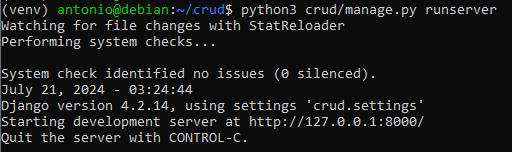
\includegraphics[]{images/s8.PNG}


\maketitle
\section{Resultados}
Os resultados incluem um aplicativo web funcional que permite  realizar operações de criação, leitura, atualização e exclusão de usuários.
Após completar todo o processo de implementação, a aplicação deve estar disponível em "http://localhost:8000". Acessando o endereço indicado este é o resultado:\\\\
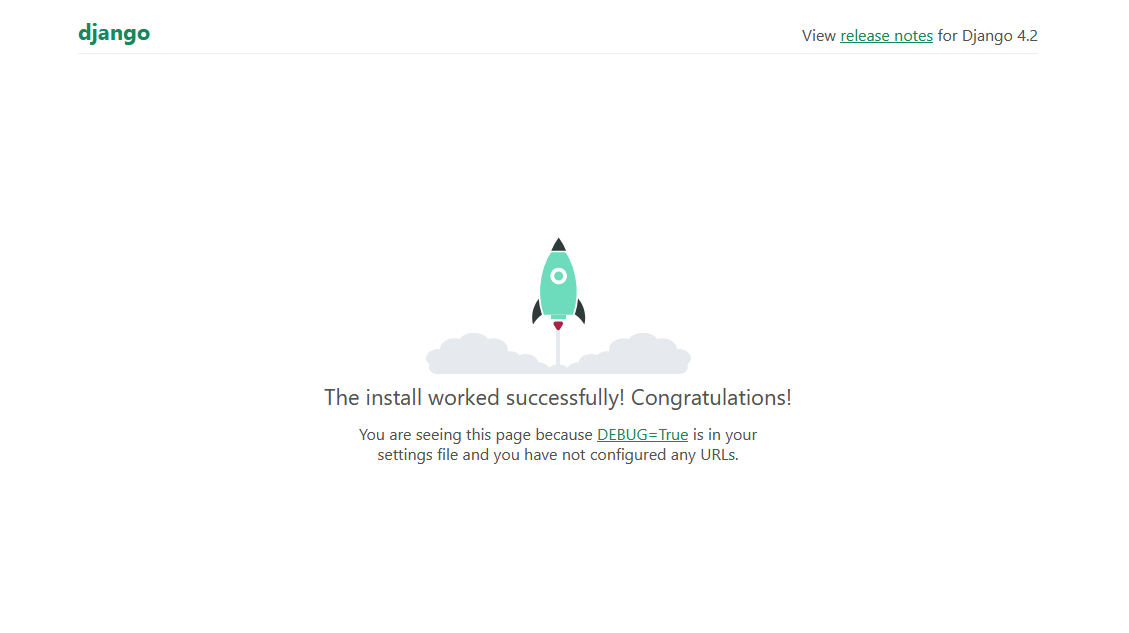
\includegraphics[width=150mm,scale=0.7]{images/s9.png}\\\\
Acessando a rota "/admin" temos o seguinte resultado:\\\\
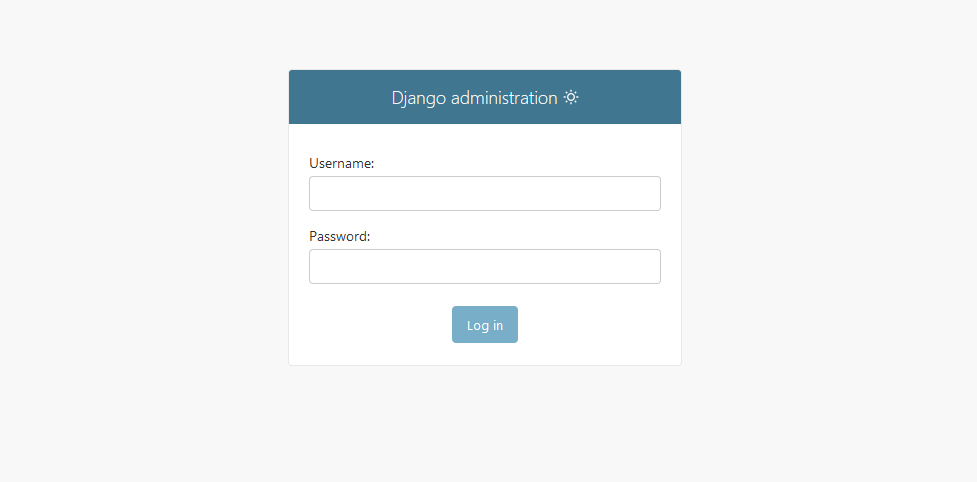
\includegraphics[width=150mm,scale=0.7]{images/s10.PNG}\\\\
Utilizando o acesso anteriormente criado para o super usuario, é possivel efetuar o login e acessar o ambiente admnistrativo.\\
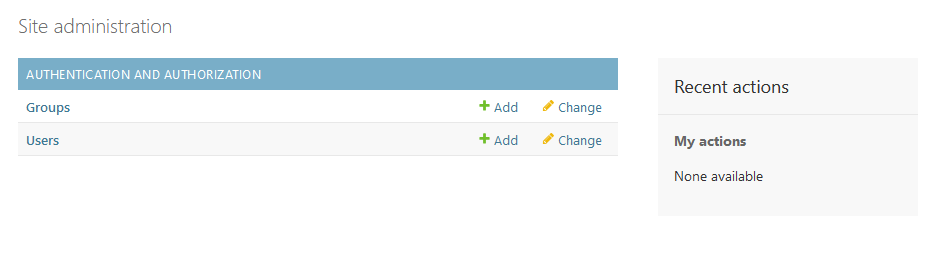
\includegraphics[width=150mm,scale=0.7]{images/s11.PNG}


\maketitle
\section{Conclusão}
Este artigo apresentou a viabilidade e a simplicidade de implementar a persistência de dados utilizando Python e Django. A abordagem passo a passo permitiu uma compreensão clara e objetiva das etapas necessárias para a construção de uma aplicação web básica, destacando o uso de ambientes virtuais, o processo de instalação do Django e a implementação de funcionalidades essenciais CRUD.\\\\
A implementação de operações de criação, leitura, atualização e exclusão (CRUD) é um requisito fundamental para o desenvolvimento de qualquer aplicação web moderna. O domínio dessas funcionalidades, aliado à robustez e escalabilidade oferecida pelo Django, proporciona ao desenvolvedor as ferramentas necessárias para criar soluções eficientes, seguras e de fácil manutenção.


\section{Referências}
\begin{enumerate}
    \item DJANGO SOFTWARE FOUNDATION. Django Documentation. 2024. Disponível em: \url{https://docs.djangoproject.com/en/5.1/}. Acesso em: 17 jul. 2024.
    \item DEBIAN LINUX. Debian Linux 5.10.0-18-amd64. Disponível em: \url{https://packages.qa.debian.org/l/linux.html}. Acesso em: 18 jul. 2024.
    \item PYTHON SOFTWARE FOUNDATION. Python 3.11.9 Release. Disponível em: \url{https://www.python.org/downloads/release/python-3119/}. Acesso em: 18 jul. 2024.
    \item MOZILLA DEVELOPER NETWORK. MDN Web Docs: Django Overview. 2024. Disponível em: \url{https://developer.mozilla.org/en-US/docs/Learn/Server-side/Django}. Acesso em: 20 jul. 2024.
    \item RAMALHO, Luciano. Python Fluente: Programação Clara, Concisa e Eficaz. 2. ed. Rio de Janeiro: Novatec Editora, 2022.
    \item DJANGO SOFTWARE FOUNDATION. Django Admin Documentation. 2024. Disponível em: \url{https://docs.djangoproject.com/en/stable/ref/contrib/admin/}. Acesso em: 22 nov. 2024.
    \item O'REILLY MEDIA. Django for Professionals: Production websites with Python and Django. 1. ed. Sebastopol: O'Reilly Media, 2020. Acesso em: 22 nov. 2024.
    \item RAHMAN, Saeed. Django 3 By Example: Build powerful and reliable web applications from scratch with Python and Django. 1. ed. Birmingham: Packt Publishing, 2020. Acesso em: 21 nov. 2024.
    \item KUBR, Martin. Pro Django: Web Application Development with Python. 1. ed. New York: Apress, 2015. Acesso em: 19 nov. 2024.
    \item GITHUB. Django Example Projects. 2024. Disponível em: \url{https://github.com/django/django-example-projects}. Acesso em: 21 nov. 2024.
    \item PYTHON SOFTWARE FOUNDATION. PIP - A package manager for Python. 2024. Disponível em: \url{https://pip.pypa.io/en/stable/}. Acesso em: 19 nov. 2024.
    \item MOZILLA DEVELOPER NETWORK. MDN Web Docs: Introduction to Django Models. 2024. Disponível em: \url{https://developer.mozilla.org/en-US/docs/Learn/Server-side/Django/Models}. Acesso em: 20 nov. 2024.
    \item SCHNEIDER, John. Test-Driven Development with Django: A practical guide to building scalable and maintainable applications. 1. ed. London: Packt Publishing, 2021. Acesso em: 20 nov. 2024.
    \item SAUNDERS, David. Mastering Django: Core Concepts. 1. ed. Birmingham: Packt Publishing, 2018. Acesso em: 18 nov. 2024.
\end{enumerate}


\end{document}